\documentclass[twoside]{book}

% Packages required by doxygen
\usepackage{fixltx2e}
\usepackage{calc}
\usepackage{doxygen}
\usepackage[export]{adjustbox} % also loads graphicx
\usepackage{graphicx}
\usepackage[utf8]{inputenc}
\usepackage{makeidx}
\usepackage{multicol}
\usepackage{multirow}
\PassOptionsToPackage{warn}{textcomp}
\usepackage{textcomp}
\usepackage[nointegrals]{wasysym}
\usepackage[table]{xcolor}

% Font selection
\usepackage[T1]{fontenc}
\usepackage[scaled=.90]{helvet}
\usepackage{courier}
\usepackage{amssymb}
\usepackage{sectsty}
\renewcommand{\familydefault}{\sfdefault}
\allsectionsfont{%
  \fontseries{bc}\selectfont%
  \color{darkgray}%
}
\renewcommand{\DoxyLabelFont}{%
  \fontseries{bc}\selectfont%
  \color{darkgray}%
}
\newcommand{\+}{\discretionary{\mbox{\scriptsize$\hookleftarrow$}}{}{}}

% Page & text layout
\usepackage{geometry}
\geometry{%
  a4paper,%
  top=2.5cm,%
  bottom=2.5cm,%
  left=2.5cm,%
  right=2.5cm%
}
\tolerance=750
\hfuzz=15pt
\hbadness=750
\setlength{\emergencystretch}{15pt}
\setlength{\parindent}{0cm}
\setlength{\parskip}{3ex plus 2ex minus 2ex}
\makeatletter
\renewcommand{\paragraph}{%
  \@startsection{paragraph}{4}{0ex}{-1.0ex}{1.0ex}{%
    \normalfont\normalsize\bfseries\SS@parafont%
  }%
}
\renewcommand{\subparagraph}{%
  \@startsection{subparagraph}{5}{0ex}{-1.0ex}{1.0ex}{%
    \normalfont\normalsize\bfseries\SS@subparafont%
  }%
}
\makeatother

% Headers & footers
\usepackage{fancyhdr}
\pagestyle{fancyplain}
\fancyhead[LE]{\fancyplain{}{\bfseries\thepage}}
\fancyhead[CE]{\fancyplain{}{}}
\fancyhead[RE]{\fancyplain{}{\bfseries\leftmark}}
\fancyhead[LO]{\fancyplain{}{\bfseries\rightmark}}
\fancyhead[CO]{\fancyplain{}{}}
\fancyhead[RO]{\fancyplain{}{\bfseries\thepage}}
\fancyfoot[LE]{\fancyplain{}{}}
\fancyfoot[CE]{\fancyplain{}{}}
\fancyfoot[RE]{\fancyplain{}{\bfseries\scriptsize Generated by Doxygen }}
\fancyfoot[LO]{\fancyplain{}{\bfseries\scriptsize Generated by Doxygen }}
\fancyfoot[CO]{\fancyplain{}{}}
\fancyfoot[RO]{\fancyplain{}{}}
\renewcommand{\footrulewidth}{0.4pt}
\renewcommand{\chaptermark}[1]{%
  \markboth{#1}{}%
}
\renewcommand{\sectionmark}[1]{%
  \markright{\thesection\ #1}%
}

% Indices & bibliography
\usepackage{natbib}
\usepackage[titles]{tocloft}
\setcounter{tocdepth}{3}
\setcounter{secnumdepth}{5}
\makeindex

% Hyperlinks (required, but should be loaded last)
\usepackage{ifpdf}
\ifpdf
  \usepackage[pdftex,pagebackref=true]{hyperref}
\else
  \usepackage[ps2pdf,pagebackref=true]{hyperref}
\fi
\hypersetup{%
  colorlinks=true,%
  linkcolor=blue,%
  citecolor=blue,%
  unicode%
}

% Custom commands
\newcommand{\clearemptydoublepage}{%
  \newpage{\pagestyle{empty}\cleardoublepage}%
}

\usepackage{caption}
\captionsetup{labelsep=space,justification=centering,font={bf},singlelinecheck=off,skip=4pt,position=top}

%===== C O N T E N T S =====

\begin{document}

% Titlepage & ToC
\hypersetup{pageanchor=false,
             bookmarksnumbered=true,
             pdfencoding=unicode
            }
\pagenumbering{alph}
\begin{titlepage}
\vspace*{7cm}
\begin{center}%
{\Large Server\+Code \\[1ex]\large 1.\+0 }\\
\vspace*{1cm}
{\large Generated by Doxygen 1.8.13}\\
\end{center}
\end{titlepage}
\clearemptydoublepage
\pagenumbering{roman}
\tableofcontents
\clearemptydoublepage
\pagenumbering{arabic}
\hypersetup{pageanchor=true}

%--- Begin generated contents ---
\chapter{Hierarchical Index}
\section{Class Hierarchy}
This inheritance list is sorted roughly, but not completely, alphabetically\+:\begin{DoxyCompactList}
\item \contentsline{section}{Gamestate}{\pageref{class_gamestate}}{}
\item \contentsline{section}{lobby}{\pageref{classlobby}}{}
\item \contentsline{section}{Map}{\pageref{class_map}}{}
\item \contentsline{section}{Message}{\pageref{class_message}}{}
\item \contentsline{section}{Player}{\pageref{class_player}}{}
\begin{DoxyCompactList}
\item \contentsline{section}{User}{\pageref{class_user}}{}
\end{DoxyCompactList}
\item \contentsline{section}{Setup\+Game}{\pageref{class_setup_game}}{}
\end{DoxyCompactList}

\chapter{Data Structure Index}
\section{Data Structures}
Here are the data structures with brief descriptions\+:\begin{DoxyCompactList}
\item\contentsline{section}{\hyperlink{class_gamestate}{Gamestate} }{\pageref{class_gamestate}}{}
\item\contentsline{section}{\hyperlink{classlobby}{lobby} }{\pageref{classlobby}}{}
\item\contentsline{section}{\hyperlink{class_map}{Map} }{\pageref{class_map}}{}
\item\contentsline{section}{\hyperlink{class_message}{Message} }{\pageref{class_message}}{}
\item\contentsline{section}{\hyperlink{class_player}{Player} }{\pageref{class_player}}{}
\item\contentsline{section}{\hyperlink{class_setup_game}{Setup\+Game} }{\pageref{class_setup_game}}{}
\item\contentsline{section}{\hyperlink{class_user}{User} }{\pageref{class_user}}{}
\end{DoxyCompactList}

\chapter{Data Structure Documentation}
\hypertarget{class_gamestate}{}\section{Gamestate Class Reference}
\label{class_gamestate}\index{Gamestate@{Gamestate}}
\subsection*{Public Member Functions}
\begin{DoxyCompactItemize}
\item 
\hyperlink{class_gamestate_af2c914e71eb7de493aa29ec74b056997}{set\+\_\+gamestate} (\$x, \$y, \$ready)
\end{DoxyCompactItemize}
\subsection*{Data Fields}
\begin{DoxyCompactItemize}
\item 
\mbox{\Hypertarget{class_gamestate_af3a16c5f0dd7a74cf9acf6a49fff73a7}\label{class_gamestate_af3a16c5f0dd7a74cf9acf6a49fff73a7}} 
{\bfseries \$x}
\item 
\mbox{\Hypertarget{class_gamestate_a77b973d137fb33212e018b042df6e3e7}\label{class_gamestate_a77b973d137fb33212e018b042df6e3e7}} 
{\bfseries \$y}
\item 
\mbox{\Hypertarget{class_gamestate_a76607f6a98433069a027747681395fb0}\label{class_gamestate_a76607f6a98433069a027747681395fb0}} 
{\bfseries \$ready}
\end{DoxyCompactItemize}


\subsection{Detailed Description}
Created by Php\+Storm.

For now its really really basic. In the future we will need to add much more variables to represent the gamestate. \hyperlink{class_user}{User}\+: johan Date\+: 08.\+10.\+2017 Time\+: 10\+:20 

Definition at line 12 of file Gamestate.\+php.



\subsection{Member Function Documentation}
\mbox{\Hypertarget{class_gamestate_af2c914e71eb7de493aa29ec74b056997}\label{class_gamestate_af2c914e71eb7de493aa29ec74b056997}} 
\index{Gamestate@{Gamestate}!set\+\_\+gamestate@{set\+\_\+gamestate}}
\index{set\+\_\+gamestate@{set\+\_\+gamestate}!Gamestate@{Gamestate}}
\subsubsection{\texorpdfstring{set\+\_\+gamestate()}{set\_gamestate()}}
{\footnotesize\ttfamily set\+\_\+gamestate (\begin{DoxyParamCaption}\item[{}]{\$x,  }\item[{}]{\$y,  }\item[{}]{\$ready }\end{DoxyParamCaption})}

Set the gamestate 
\begin{DoxyParams}{Parameters}
{\em \$x} & \\
\hline
{\em \$y} & \\
\hline
{\em \$ready} & \\
\hline
\end{DoxyParams}


Definition at line 24 of file Gamestate.\+php.



The documentation for this class was generated from the following file\+:\begin{DoxyCompactItemize}
\item 
json\+\_\+helper/Gamestate.\+php\end{DoxyCompactItemize}

\hypertarget{classlobby}{}\section{lobby Class Reference}
\label{classlobby}\index{lobby@{lobby}}
\subsection*{Public Member Functions}
\begin{DoxyCompactItemize}
\item 
\hyperlink{classlobby_a0501effa0478716d61dbc830ae7ac0c0}{set\+\_\+lobby} (\$leader\+ID, \$leader\+Username, \$gamemode, \$game\+ID, \$opponent\+ID, \$opponent\+Username)
\end{DoxyCompactItemize}
\subsection*{Data Fields}
\begin{DoxyCompactItemize}
\item 
\mbox{\Hypertarget{classlobby_ae011f12226aa240566aa5b17c6a905a4}\label{classlobby_ae011f12226aa240566aa5b17c6a905a4}} 
{\bfseries \$leader\+ID}
\item 
\mbox{\Hypertarget{classlobby_a4c162cc429c50427e1e4aef5f7567efa}\label{classlobby_a4c162cc429c50427e1e4aef5f7567efa}} 
{\bfseries \$leader\+Username}
\item 
\mbox{\Hypertarget{classlobby_a3fd98457ff4f3251dfac6d6a01965f98}\label{classlobby_a3fd98457ff4f3251dfac6d6a01965f98}} 
{\bfseries \$gamemode}
\item 
\mbox{\Hypertarget{classlobby_aa27e936ca36f62a3e0478528c5274356}\label{classlobby_aa27e936ca36f62a3e0478528c5274356}} 
{\bfseries \$game\+ID}
\item 
\mbox{\Hypertarget{classlobby_ad0db2a880e262730fabe6a221910aefc}\label{classlobby_ad0db2a880e262730fabe6a221910aefc}} 
{\bfseries \$opponent\+ID}
\item 
\mbox{\Hypertarget{classlobby_adf1f61ed1a8f7f727ad3b321bfd00cc1}\label{classlobby_adf1f61ed1a8f7f727ad3b321bfd00cc1}} 
{\bfseries \$opponent\+Username}
\end{DoxyCompactItemize}


\subsection{Detailed Description}
Created by Php\+Storm. \hyperlink{class_user}{User}\+: johan Date\+: 05.\+11.\+2017 Time\+: 17\+:32 

Definition at line 9 of file Lobby.\+php.



\subsection{Member Function Documentation}
\mbox{\Hypertarget{classlobby_a0501effa0478716d61dbc830ae7ac0c0}\label{classlobby_a0501effa0478716d61dbc830ae7ac0c0}} 
\index{lobby@{lobby}!set\+\_\+lobby@{set\+\_\+lobby}}
\index{set\+\_\+lobby@{set\+\_\+lobby}!lobby@{lobby}}
\subsubsection{\texorpdfstring{set\+\_\+lobby()}{set\_lobby()}}
{\footnotesize\ttfamily set\+\_\+lobby (\begin{DoxyParamCaption}\item[{}]{\$leader\+ID,  }\item[{}]{\$leader\+Username,  }\item[{}]{\$gamemode,  }\item[{}]{\$game\+ID,  }\item[{}]{\$opponent\+ID,  }\item[{}]{\$opponent\+Username }\end{DoxyParamCaption})}

Set the lobby 
\begin{DoxyParams}{Parameters}
{\em \$leader\+ID} & \\
\hline
{\em \$leader\+Username} & \\
\hline
{\em \$gamemode} & \\
\hline
{\em \$game\+ID} & \\
\hline
{\em \$opponent\+ID} & \\
\hline
{\em \$opponent\+Username} & \\
\hline
\end{DoxyParams}


Definition at line 27 of file Lobby.\+php.



The documentation for this class was generated from the following file\+:\begin{DoxyCompactItemize}
\item 
json\+\_\+helper/Lobby.\+php\end{DoxyCompactItemize}

\hypertarget{class_map}{}\section{Map Class Reference}
\label{class_map}\index{Map@{Map}}
\subsection*{Public Member Functions}
\begin{DoxyCompactItemize}
\item 
\hyperlink{class_map_a9fe8c6be6b6ef95747e4eb3ab49c2c10}{set\+\_\+map} (\$map\+ID, \$map\+Name, \$map\+Description, \$author)
\end{DoxyCompactItemize}
\subsection*{Data Fields}
\begin{DoxyCompactItemize}
\item 
\mbox{\Hypertarget{class_map_ace12b3203ac5df07d868adda1786188e}\label{class_map_ace12b3203ac5df07d868adda1786188e}} 
{\bfseries \$map\+ID}
\item 
\mbox{\Hypertarget{class_map_a5d5eba19afce030ab95fc126746396b4}\label{class_map_a5d5eba19afce030ab95fc126746396b4}} 
{\bfseries \$map\+Name}
\item 
\mbox{\Hypertarget{class_map_a9eefab63676fcdc4712153055d66c7a3}\label{class_map_a9eefab63676fcdc4712153055d66c7a3}} 
{\bfseries \$map\+Description}
\item 
\mbox{\Hypertarget{class_map_ac35b828f7d4064a7c9f849c255468ee3}\label{class_map_ac35b828f7d4064a7c9f849c255468ee3}} 
{\bfseries \$author}
\end{DoxyCompactItemize}


\subsection{Detailed Description}
Created by Php\+Storm. This is just a holder for the \hyperlink{class_map}{Map}. It helps when we want to convert it into a J\+S\+ON

\hyperlink{class_user}{User}\+: johan Date\+: 12.\+10.\+2017 Time\+: 15\+:58 

Definition at line 12 of file Map.\+php.



\subsection{Member Function Documentation}
\mbox{\Hypertarget{class_map_a9fe8c6be6b6ef95747e4eb3ab49c2c10}\label{class_map_a9fe8c6be6b6ef95747e4eb3ab49c2c10}} 
\index{Map@{Map}!set\+\_\+map@{set\+\_\+map}}
\index{set\+\_\+map@{set\+\_\+map}!Map@{Map}}
\subsubsection{\texorpdfstring{set\+\_\+map()}{set\_map()}}
{\footnotesize\ttfamily set\+\_\+map (\begin{DoxyParamCaption}\item[{}]{\$map\+ID,  }\item[{}]{\$map\+Name,  }\item[{}]{\$map\+Description,  }\item[{}]{\$author }\end{DoxyParamCaption})}

set the map 
\begin{DoxyParams}{Parameters}
{\em \$map\+ID} & \\
\hline
{\em \$map\+Name} & \\
\hline
{\em \$map\+Description} & \\
\hline
{\em \$author} & \\
\hline
\end{DoxyParams}


Definition at line 26 of file Map.\+php.



The documentation for this class was generated from the following file\+:\begin{DoxyCompactItemize}
\item 
json\+\_\+helper/Map.\+php\end{DoxyCompactItemize}

\hypertarget{class_message}{}\section{Message Class Reference}
\label{class_message}\index{Message@{Message}}
\subsection*{Public Member Functions}
\begin{DoxyCompactItemize}
\item 
\hyperlink{class_message_a236d96a999436f667b75462621635329}{set\+\_\+message} (\$from\+ID, \$from\+Username, \$message)
\end{DoxyCompactItemize}
\subsection*{Data Fields}
\begin{DoxyCompactItemize}
\item 
\mbox{\Hypertarget{class_message_a5c507155944f7032089f120efa5f8f36}\label{class_message_a5c507155944f7032089f120efa5f8f36}} 
{\bfseries \$message\+ID}
\item 
\mbox{\Hypertarget{class_message_ad8dc72dc170b758cbb59b827cdb3aa31}\label{class_message_ad8dc72dc170b758cbb59b827cdb3aa31}} 
{\bfseries \$from\+ID}
\item 
\mbox{\Hypertarget{class_message_a34edec9dd5007ed33c8a628a7c4e907a}\label{class_message_a34edec9dd5007ed33c8a628a7c4e907a}} 
{\bfseries \$from\+Username}
\item 
\mbox{\Hypertarget{class_message_abf17cb2dba2ed17cb28aa5f37deb5293}\label{class_message_abf17cb2dba2ed17cb28aa5f37deb5293}} 
{\bfseries \$message}
\end{DoxyCompactItemize}


\subsection{Detailed Description}
Created by Php\+Storm. \hyperlink{class_user}{User}\+: johan Date\+: 02.\+11.\+2017 Time\+: 18\+:14 

Definition at line 9 of file Message.\+php.



\subsection{Member Function Documentation}
\mbox{\Hypertarget{class_message_a236d96a999436f667b75462621635329}\label{class_message_a236d96a999436f667b75462621635329}} 
\index{Message@{Message}!set\+\_\+message@{set\+\_\+message}}
\index{set\+\_\+message@{set\+\_\+message}!Message@{Message}}
\subsubsection{\texorpdfstring{set\+\_\+message()}{set\_message()}}
{\footnotesize\ttfamily set\+\_\+message (\begin{DoxyParamCaption}\item[{}]{\$from\+ID,  }\item[{}]{\$from\+Username,  }\item[{}]{\$message }\end{DoxyParamCaption})}

sett the message 
\begin{DoxyParams}{Parameters}
{\em \$from\+ID} & \\
\hline
{\em \$from\+Username} & \\
\hline
{\em \$message} & \\
\hline
\end{DoxyParams}


Definition at line 22 of file Message.\+php.



The documentation for this class was generated from the following file\+:\begin{DoxyCompactItemize}
\item 
json\+\_\+helper/Message.\+php\end{DoxyCompactItemize}

\hypertarget{class_player}{}\section{Player Class Reference}
\label{class_player}\index{Player@{Player}}
Inheritance diagram for Player\+:\begin{figure}[H]
\begin{center}
\leavevmode
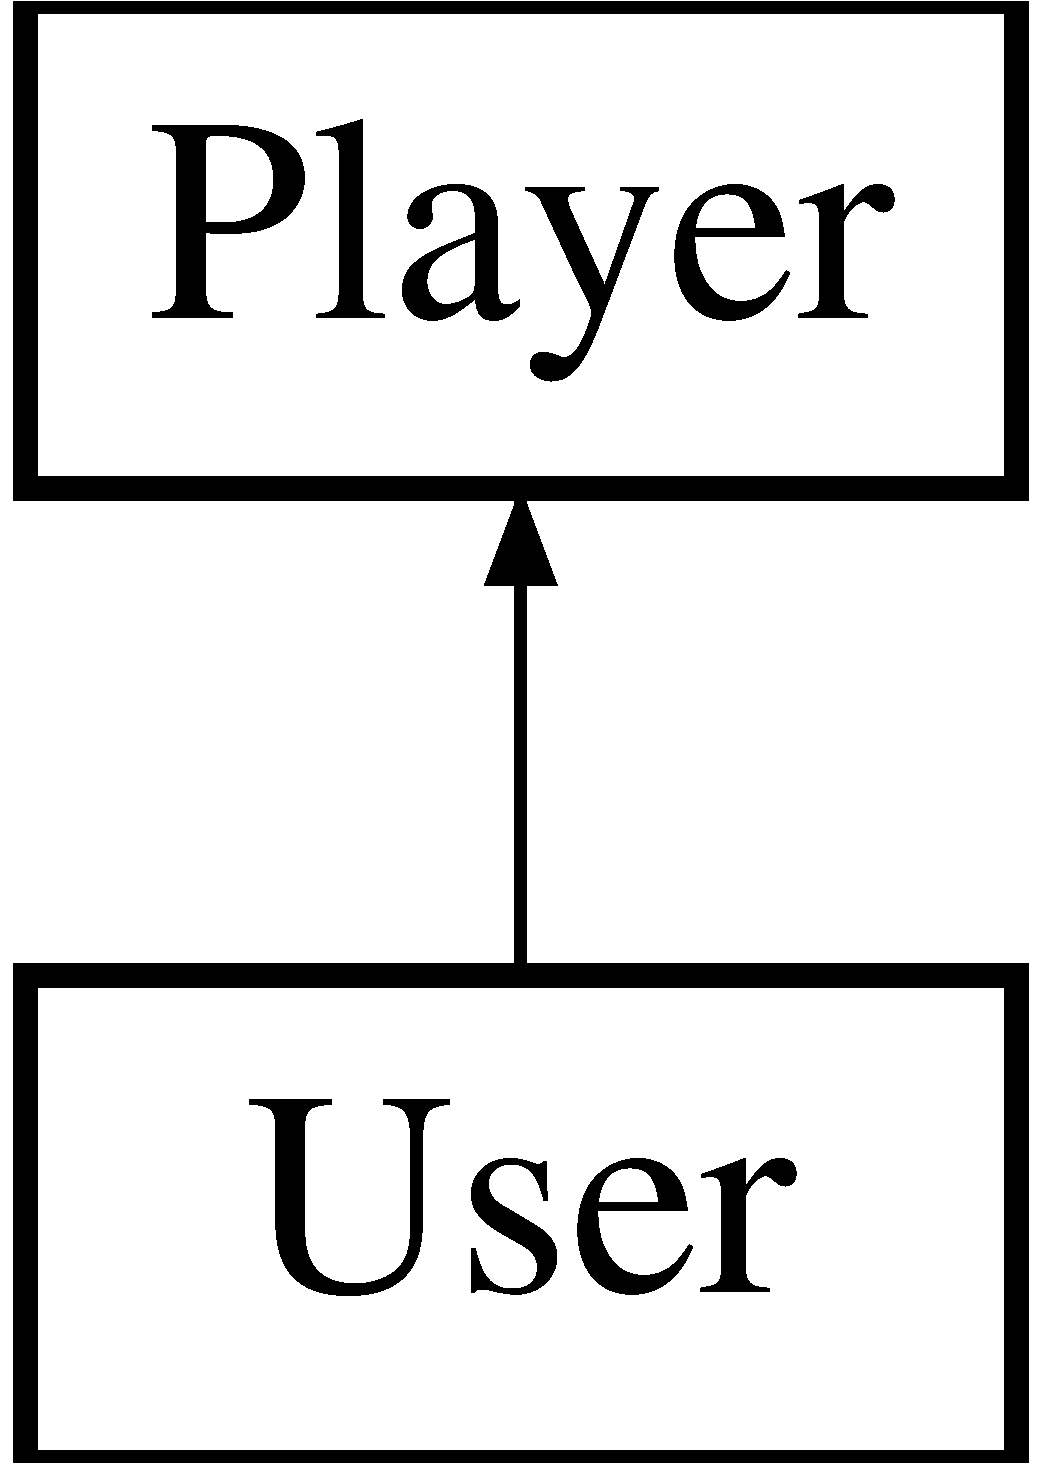
\includegraphics[height=2.000000cm]{class_player}
\end{center}
\end{figure}
\subsection*{Public Member Functions}
\begin{DoxyCompactItemize}
\item 
\hyperlink{class_player_a29bdabbd71ff2caf58838b676e8734b2}{set\+\_\+player} (\$Player\+ID, \$username, \$message)
\end{DoxyCompactItemize}
\subsection*{Data Fields}
\begin{DoxyCompactItemize}
\item 
\mbox{\Hypertarget{class_player_a0eb82aa5f81cf845de4b36cd653c42cf}\label{class_player_a0eb82aa5f81cf845de4b36cd653c42cf}} 
{\bfseries \$username}
\item 
\mbox{\Hypertarget{class_player_a9a4de079dad1eca41a99f7c18ab49485}\label{class_player_a9a4de079dad1eca41a99f7c18ab49485}} 
{\bfseries \$\+Player\+ID}
\item 
\mbox{\Hypertarget{class_player_abf17cb2dba2ed17cb28aa5f37deb5293}\label{class_player_abf17cb2dba2ed17cb28aa5f37deb5293}} 
{\bfseries \$message}
\end{DoxyCompactItemize}


\subsection{Detailed Description}


Definition at line 2 of file Player.\+php.



\subsection{Member Function Documentation}
\mbox{\Hypertarget{class_player_a29bdabbd71ff2caf58838b676e8734b2}\label{class_player_a29bdabbd71ff2caf58838b676e8734b2}} 
\index{Player@{Player}!set\+\_\+player@{set\+\_\+player}}
\index{set\+\_\+player@{set\+\_\+player}!Player@{Player}}
\subsubsection{\texorpdfstring{set\+\_\+player()}{set\_player()}}
{\footnotesize\ttfamily set\+\_\+player (\begin{DoxyParamCaption}\item[{}]{\$\+Player\+ID,  }\item[{}]{\$username,  }\item[{}]{\$message }\end{DoxyParamCaption})}

set the player 
\begin{DoxyParams}{Parameters}
{\em \$\+Player\+ID} & \\
\hline
{\em \$username} & \\
\hline
{\em \$message} & \\
\hline
\end{DoxyParams}


Definition at line 13 of file Player.\+php.



The documentation for this class was generated from the following file\+:\begin{DoxyCompactItemize}
\item 
json\+\_\+helper/Player.\+php\end{DoxyCompactItemize}

\hypertarget{class_setup_game}{}\section{Setup\+Game Class Reference}
\label{class_setup_game}\index{Setup\+Game@{Setup\+Game}}
\subsection*{Public Member Functions}
\begin{DoxyCompactItemize}
\item 
\hyperlink{class_setup_game_a075e4bec4b509da98abb32143f175e0e}{set\+\_\+setup} (\$race1, \$race2, \$map\+ID, \$leader\+ID, \$opponent\+ID, \$game\+ID, \$gamemode)
\end{DoxyCompactItemize}
\subsection*{Data Fields}
\begin{DoxyCompactItemize}
\item 
\mbox{\Hypertarget{class_setup_game_ae011f12226aa240566aa5b17c6a905a4}\label{class_setup_game_ae011f12226aa240566aa5b17c6a905a4}} 
{\bfseries \$leader\+ID}
\item 
\mbox{\Hypertarget{class_setup_game_af8613490d33c93235d9753a9839bddf9}\label{class_setup_game_af8613490d33c93235d9753a9839bddf9}} 
{\bfseries \$race1}
\item 
\mbox{\Hypertarget{class_setup_game_a0857d41d4220fe1d00a157cd50913313}\label{class_setup_game_a0857d41d4220fe1d00a157cd50913313}} 
{\bfseries \$race2}
\item 
\mbox{\Hypertarget{class_setup_game_aa27e936ca36f62a3e0478528c5274356}\label{class_setup_game_aa27e936ca36f62a3e0478528c5274356}} 
{\bfseries \$game\+ID}
\item 
\mbox{\Hypertarget{class_setup_game_ace12b3203ac5df07d868adda1786188e}\label{class_setup_game_ace12b3203ac5df07d868adda1786188e}} 
{\bfseries \$map\+ID}
\item 
\mbox{\Hypertarget{class_setup_game_ad0db2a880e262730fabe6a221910aefc}\label{class_setup_game_ad0db2a880e262730fabe6a221910aefc}} 
{\bfseries \$opponent\+ID}
\item 
\mbox{\Hypertarget{class_setup_game_a3fd98457ff4f3251dfac6d6a01965f98}\label{class_setup_game_a3fd98457ff4f3251dfac6d6a01965f98}} 
{\bfseries \$gamemode}
\end{DoxyCompactItemize}


\subsection{Detailed Description}
Created by Php\+Storm. \hyperlink{class_user}{User}\+: johan Date\+: 05.\+11.\+2017 Time\+: 19\+:05 

Definition at line 9 of file Setup\+Game.\+php.



\subsection{Member Function Documentation}
\mbox{\Hypertarget{class_setup_game_a075e4bec4b509da98abb32143f175e0e}\label{class_setup_game_a075e4bec4b509da98abb32143f175e0e}} 
\index{Setup\+Game@{Setup\+Game}!set\+\_\+setup@{set\+\_\+setup}}
\index{set\+\_\+setup@{set\+\_\+setup}!Setup\+Game@{Setup\+Game}}
\subsubsection{\texorpdfstring{set\+\_\+setup()}{set\_setup()}}
{\footnotesize\ttfamily set\+\_\+setup (\begin{DoxyParamCaption}\item[{}]{\$race1,  }\item[{}]{\$race2,  }\item[{}]{\$map\+ID,  }\item[{}]{\$leader\+ID,  }\item[{}]{\$opponent\+ID,  }\item[{}]{\$game\+ID,  }\item[{}]{\$gamemode }\end{DoxyParamCaption})}

Set the setup 
\begin{DoxyParams}{Parameters}
{\em \$race1} & \\
\hline
{\em \$race2} & \\
\hline
{\em \$map\+ID} & \\
\hline
{\em \$leader\+ID} & \\
\hline
{\em \$opponent\+ID} & \\
\hline
{\em \$game\+ID} & \\
\hline
{\em \$gamemode} & \\
\hline
\end{DoxyParams}


Definition at line 31 of file Setup\+Game.\+php.



The documentation for this class was generated from the following file\+:\begin{DoxyCompactItemize}
\item 
json\+\_\+helper/Setup\+Game.\+php\end{DoxyCompactItemize}

\hypertarget{class_user}{}\section{User Class Reference}
\label{class_user}\index{User@{User}}
Inheritance diagram for User\+:\begin{figure}[H]
\begin{center}
\leavevmode
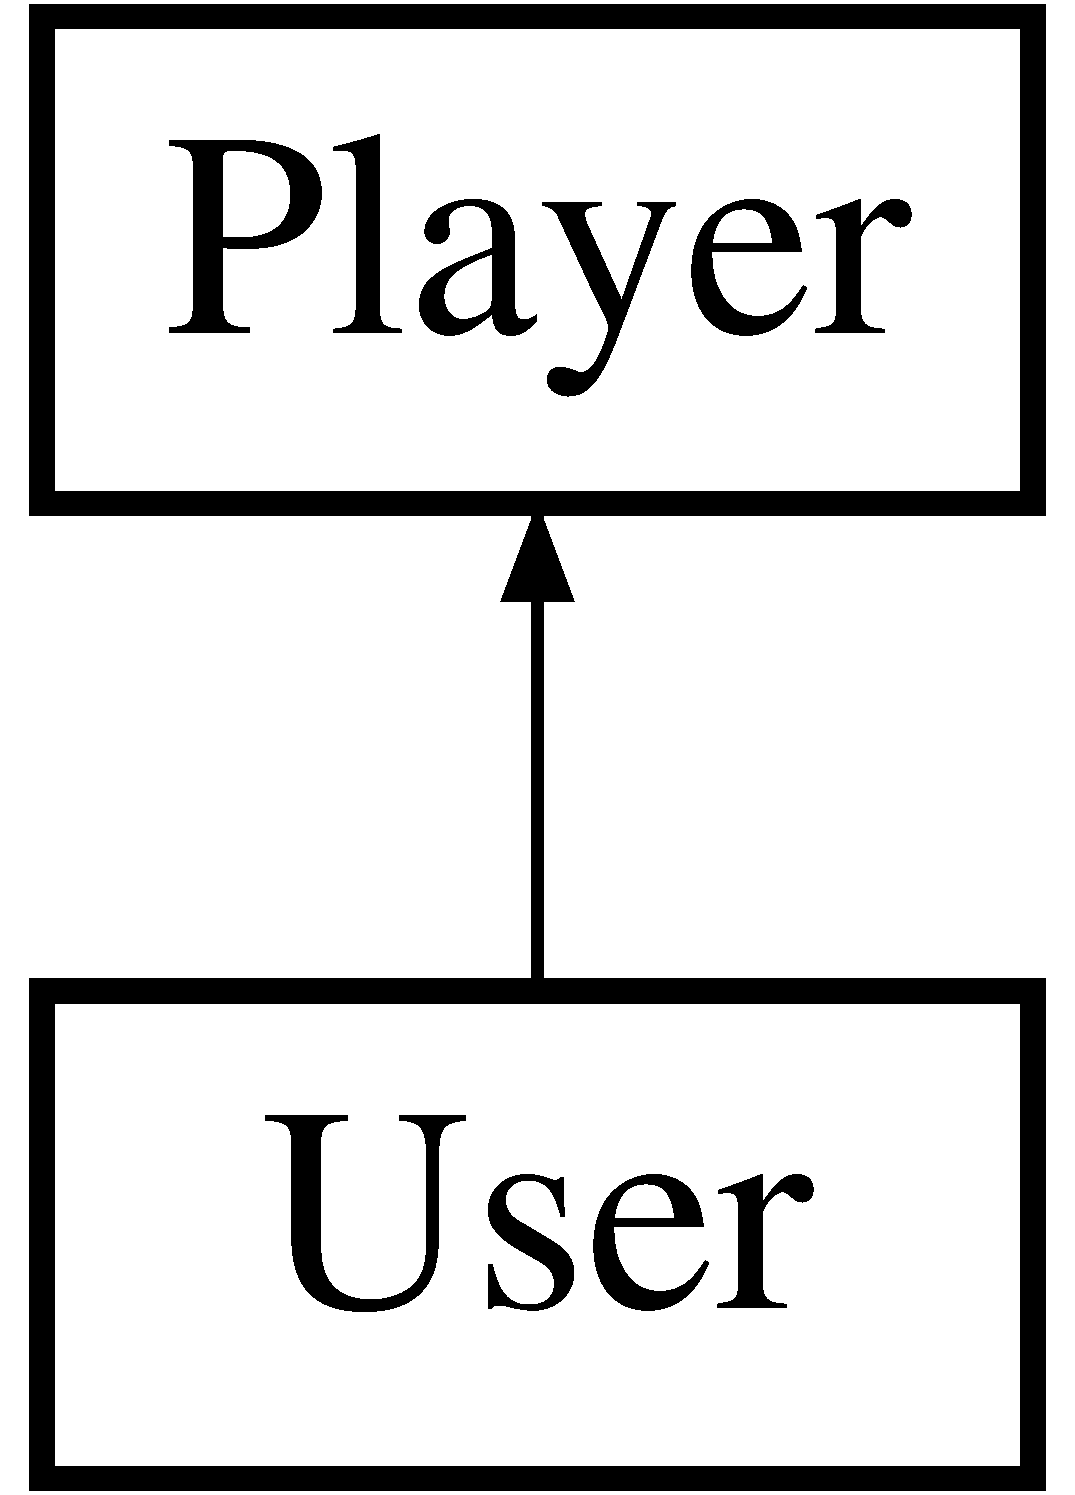
\includegraphics[height=2.000000cm]{class_user}
\end{center}
\end{figure}
\subsection*{Public Member Functions}
\begin{DoxyCompactItemize}
\item 
\hyperlink{class_user_a8cefa83861ded23e81667e5ba3a98702}{set\+\_\+user} (\$player\+ID, \$username, \$message, \$number\+Wins, \$number\+Loss, \$image\+ID)
\end{DoxyCompactItemize}
\subsection*{Data Fields}
\begin{DoxyCompactItemize}
\item 
\mbox{\Hypertarget{class_user_a4a9417bc21ce9ff476de702c9b007326}\label{class_user_a4a9417bc21ce9ff476de702c9b007326}} 
{\bfseries \$number\+Wins}
\item 
\mbox{\Hypertarget{class_user_a6c280f09f0d796423df08262a813a632}\label{class_user_a6c280f09f0d796423df08262a813a632}} 
{\bfseries \$number\+Loss}
\item 
\mbox{\Hypertarget{class_user_a083e40d42ed789f034faea0f132b86fb}\label{class_user_a083e40d42ed789f034faea0f132b86fb}} 
{\bfseries \$image\+ID}
\end{DoxyCompactItemize}


\subsection{Detailed Description}
Created by Php\+Storm. \hyperlink{class_user}{User}\+: johan Date\+: 23.\+10.\+2017 Time\+: 12\+:15 

Definition at line 10 of file User.\+php.



\subsection{Member Function Documentation}
\mbox{\Hypertarget{class_user_a8cefa83861ded23e81667e5ba3a98702}\label{class_user_a8cefa83861ded23e81667e5ba3a98702}} 
\index{User@{User}!set\+\_\+user@{set\+\_\+user}}
\index{set\+\_\+user@{set\+\_\+user}!User@{User}}
\subsubsection{\texorpdfstring{set\+\_\+user()}{set\_user()}}
{\footnotesize\ttfamily set\+\_\+user (\begin{DoxyParamCaption}\item[{}]{\$player\+ID,  }\item[{}]{\$username,  }\item[{}]{\$message,  }\item[{}]{\$number\+Wins,  }\item[{}]{\$number\+Loss,  }\item[{}]{\$image\+ID }\end{DoxyParamCaption})}

Set the user. 
\begin{DoxyParams}{Parameters}
{\em \$player\+ID} & \\
\hline
{\em \$username} & \\
\hline
{\em \$message} & \\
\hline
{\em \$number\+Wins} & \\
\hline
{\em \$number\+Loss} & \\
\hline
{\em \$image\+ID} & \\
\hline
\end{DoxyParams}


Definition at line 26 of file User.\+php.



The documentation for this class was generated from the following file\+:\begin{DoxyCompactItemize}
\item 
json\+\_\+helper/User.\+php\end{DoxyCompactItemize}

%--- End generated contents ---

% Index
\backmatter
\newpage
\phantomsection
\clearemptydoublepage
\addcontentsline{toc}{chapter}{Index}
\printindex

\end{document}
